\chapter{Graphrepräsentationen von Bildern}

planarer Graph (MUSS NICHT UNBEDINGT SEIN), gegenbeispiel, ist aber auch egal

\section{Kantengewichte}

Kantengewichte werden ermittelt aus der euklidischen Distanz der Zentren zweier adjazenter Regionen $\left\|\gls{p}\left(v\right) - \gls{p}\left(u\right)\right\|_2$.
Distanz entspricht aber nicht der üblichen Bedeutung von Kantengewichten auf Graphen.
Je höher das Gewicht, desto ähnlicher bzw.\ näher sind zwei Knoten.

Ein üblicher Weg die Distanz zweier Knoten zueinander als Kantengewicht darzustellen ist über einen gewichteten \emph{Gaussian-Kernel}~\cite{Shuman}
\begin{equation}
  \gls{w}\left(v, u\right) = \exp\left(-\frac{\left\|\gls{p}\left(v\right) - \gls{p}\left(u\right)\right\|_2}{2\theta^2}\right)
\end{equation}

falls $v \gls{adj} u$ und einem Parameter $\theta \in \gls{R}$.

Die Wahl von $\theta$ ist dabei abhängig von der Ausdehnung der Distanzen eines Graphen.

\begin{center}
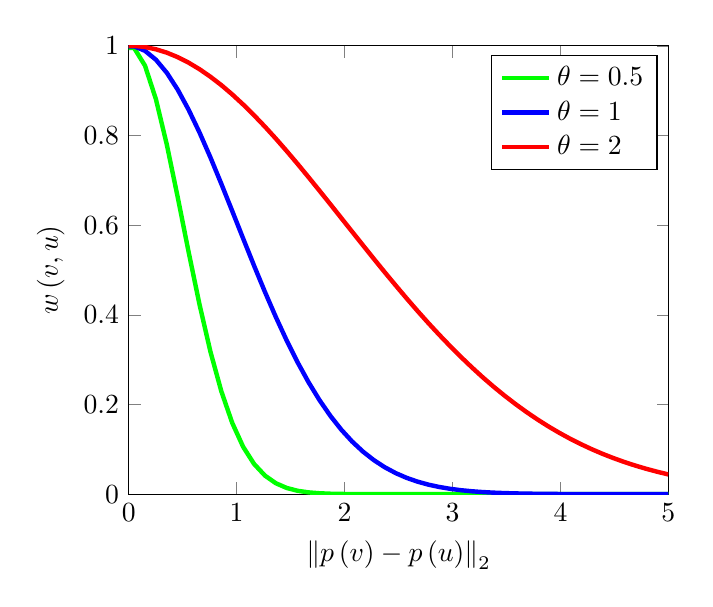
\begin{tikzpicture}
  \begin{axis}[xmax=5,
               xmin=0,
               ymin=0,
               ymax=1,
               xlabel={$\left\|\gls{p}\left(v\right) - \gls{p}\left(u\right)\right\|_2$},
               ylabel={$\gls{w}\left(v, u\right)$},
               legend cell align=left]
    \addplot [samples=100, ultra thick, green] {exp(-(x^2)/(2*0.5^2))};
    \addlegendentry{$\theta = 0.5$}
    \addplot [samples=100, ultra thick, blue] {exp(-(x^2)/(2*1^2))};
    \addlegendentry{$\theta = 1$}
    \addplot [samples=100, ultra thick, red] {exp(-(x^2)/(2*2^2))};
    \addlegendentry{$\theta = 2$}
  \end{axis}
\end{tikzpicture}
\end{center}
